\documentclass[12pt,letterpaper]{article}
\usepackage[latin1]{inputenc}
\usepackage{amsmath}
\usepackage{amsfonts}
\usepackage{amssymb}

% the above packages are the "base"

\usepackage{graphicx}

\usepackage{hyperref} % enable links within pdf
\hypersetup{colorlinks = true, linkcolor = black, urlcolor = blue}

 \usepackage[hang,flushmargin]{footmisc} % don't indent footnotes

\usepackage{ragged2e} % for justify{}
% Define a function to make a Ben-specific font :-)
 \newenvironment{ben}{\quote\justify\fontfamily{cmtt}\selectfont\small}{\par}

\setcounter{secnumdepth}{0}  % don't number sections (stars not needed)


%%%%%%%%%%%%%%%%%%%%%%%%%%%%%%%%%

\author{}
\title{Structuring your project}
\date{}

\begin{document}

\maketitle
% \tableofcontents
% \pagebreak

The general recommendations of this section in regards to establishing a consistent structure for your project should apply whether or not you plan to use version control software to manage your project or not.
For example, the recommendations apply equally if you plan to use \texttt{Dropbox} or the equivalent (which you should \emph{most definitely} be using if you're not going to use version control software).

\section{Developing a project mindset} \label{projectmindset}

Like many grad students, I finished my thesis with
\begin{itemize}
	\item one master folder called \texttt{Data} containing a bunch of sub-folders containing the various data sets (mostly Excel and CSV files) and some relational databases (Microsoft Access) that I'd collected or collated over the years;
	\item one master folder called \texttt{Rcodes} containing a bunch of sub-folders within it (each with a different project (chapter) and/or set of analyses of some set of my data);
	\item one master folder called \texttt{Mathematica} that similarly contained a bunch of sub-folders for various projects;
	\item one master folder called \texttt{Manuscripts} that contained all the papers and chapters I'd attempted or completed;
\end{itemize}
and a bunch more similar folders all variously named and ``type-specific'' within my overall \texttt{Research} folder.
You might currently have something similar for your thesis work (Fig.~\ref{fig:old_figs}).

Turns out that's a poor way to organize your work for a variety of reasons, including the ease of backing-up new data and code;
the ease and efficiency with which you might expand, modify or branch off of your prior work;
and even the simple reproducability of past work (by yourself down the road, or by someone else for whom you'll have to pull together all the necessary parts).

I now organize my work using a \emph{project mindset}.  I don't do this for each and every project idea or analysis I try out, but I do use it for ``definitely doing this'' (i.e.  planned-out papers (thesis chapters)) and collaborative projects.
By project mindset, I mean that (almost) everything associated with a given project is contained in one folder.
I do still use a combination of \texttt{Git} and \texttt{Dropbox} to organize my projects based on my plans for projects\footnote{For example, whether I plan to make the entire project publicly available.} and collaboraton needs, but within each of \texttt{Dropbox} and \texttt{Git} I have my project folders organized within a master folder.\footnote{Note that you're asking for trouble if you put a \texttt{Git} folder within your \texttt{Dropbox} or \texttt{GoogleDrive} folder, or vice versa.}

All that said, defining ``a project'' can get difficult (esp. within your thesis work), so a fair bit of forethought is often needed.
We'll definitely talk about this as a group in class.
It's not trivial, but becomes quicker with time and seeing what others do.

\begin{ben}
	\textit{Ben adds:}
		I also use project mindset to organize my folders.
		Something I like about project mindset is that it encourages what you might call \emph{deliverables-based} thinking.
		By identifying and naming the "definitely doing this" projects, I am encouraged to consider my priorities, both within and among projects.

		For each project I am forced to think clearly about what the project is fundamentally about by having to name the folder.
		Asking "what should this project folder (or Git repo) be called?" (and insisting on an \emph{informative name})\footnote{Naming conventions are something we'll come back to when we talk about good coding practices.}
		is pretty close to asking "what is this project about?"
		So a project mindset supports clear thinking.

		I also find that a project mindset promotes better time management.
		For instance, all my project folders are contained within three superfolders: Active, Complete and Archive.
		The folders within Complete are named with dates and brief titles of publication.
		The Active folder contains stuff I am working on right now, that has not "shipped" yet.
		Archive is for stuff that is on the back-burner.

		In this setup, the project folders within the Active folder - each with a name that reminds me of the objective for that project - becomes a kind of high-level to-do list.
		The goal is to be able to one day drag those folders from Active to Complete.
		Crucially, if the Active folder gets too full, I know I will not be able to do succeed in moving project folders because my attention has become too divided.
		So then I ask myself which are the most important few projects to me, and drag the rest to the Archive folder.
		It's not that I can't do them later.
		It is just recognizing that (a) they are not done yet, and (b) they are not the first, second or even third priority.
		If both (a) and (b) are true, into the Archive folder they go!
		OK, back to Mark, and the structure of an individual project folder.
\end{ben}




\section{Structuring your Project folder / Repository} \label{projectfolder}

For most projects, within each project folder, I usually have the following sub-folders:

\begin{tabular}{ll}
 \texttt{data} & the original (and cleaned) data required for the project\\
 \texttt{code} & all the scripts needed to perform the analyses \\
 \texttt{results} & all the output of the analyses \\
 \texttt{biblio} & bibliographic files\\
 \texttt{figs} & final figures (and tables) that go into the manuscript\\
 \texttt{manuscript} & manuscript(s) derived from the project\\
 \texttt{pdfs} & collection of relevant papers, manuals, etc.\\
\end{tabular}

\noindent
The first three (\texttt{data}, \texttt{code} and \texttt{output}) are definites for any project (repository) that I plan to make public (e.g., on GitHub).
For such public repositories, I do not include the other four folders.
I use \texttt{figs}, \texttt{manuscript}, \texttt{biblio} and \texttt{pdfs} for manuscript-writing ``projects'' (which I place in an \texttt{InPrep} manuscripts-only sub-folder within my master \texttt{Git} folder).
The contents of \texttt{figs} differs from the rough-and-dirty figures I save into the \texttt{output} folder.
Sometimes \texttt{tables} get their own folder.
Within \texttt{code} I might have an \texttt{R} and a \texttt{Mathematica} folder, as relevant.
Note that \texttt{data} contains both the untouched original data\footnote{Leaving your original data as untouched as possible is something we'll come back to during Coding Best Practices} and the clearly-identified cleaned or otherwise derived data (for ease of subsequent access).

\begin{ben}
	\textit{Ben says}: My sub-folder structure is similar, with variations depending on the project and preferences. For example, my reference manager of choice keeps all my pdfs in one place, so instead of having a pdfs folder in each project folder, I have "folders" for each project within my reference manager. Either way, the same goal is achieved: a logical hierarchical structure that makes it easy to find and keep the various pieces of a project. Back to you Mark.
\end{ben}

Most of the time when using \texttt{Git} you'll have one \emph{repository} associated with each one of your \emph{projects}.  A \emph{repository} is thus synonymous with a \emph{project folder}.  When using \texttt{Git} you'll also have a few other files within the repository: a \texttt{README.md} file and a \texttt{.gitignore} file.  If you're using \texttt{R-Studio} in combination with \texttt{Git} (as we will in this course), then you may also have an \texttt{.Rproj} file in the repository.  It's good practice to have a \texttt{README.md} file in each of the ``important'' folders, describing what in them.

\begin{figure}[!h]
	\centering
	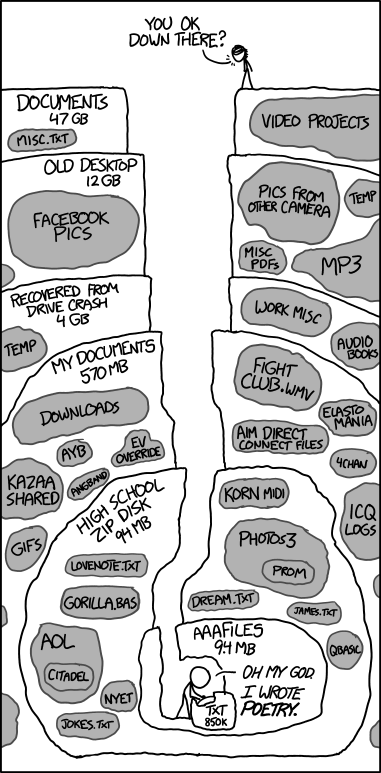
\includegraphics[width=0.5\linewidth]{figs/xkcd_old_files}
	\caption{Old files (source: \url{http://xkcd.com/1360/})}
	\label{fig:old_figs}
\end{figure}

\end{document}
